\chapter{Implementation}
In this chapter, the implementation details are talked about. The technologies that used are described, alongside the justification for selecting them. While the system has coherently isolated components, to be specific a subsystem of Data Gathering, Neural Translation Model and a Visualization Interface, each with different design strategies and implementation approach.

\begin{figure}[h]
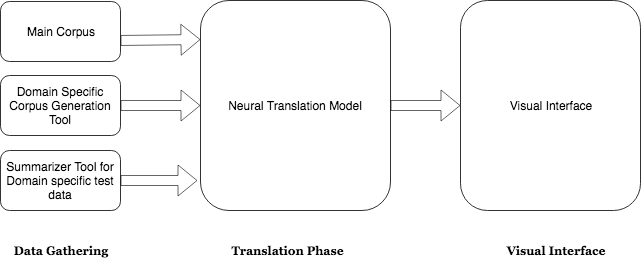
\includegraphics[width=\textwidth]{figures/maindesign.png}
\caption{System Components} \label{system}
\end{figure}

\section{Data Gathering}
\subsection{Dataset for Fine Tuning}
\begin{figure}
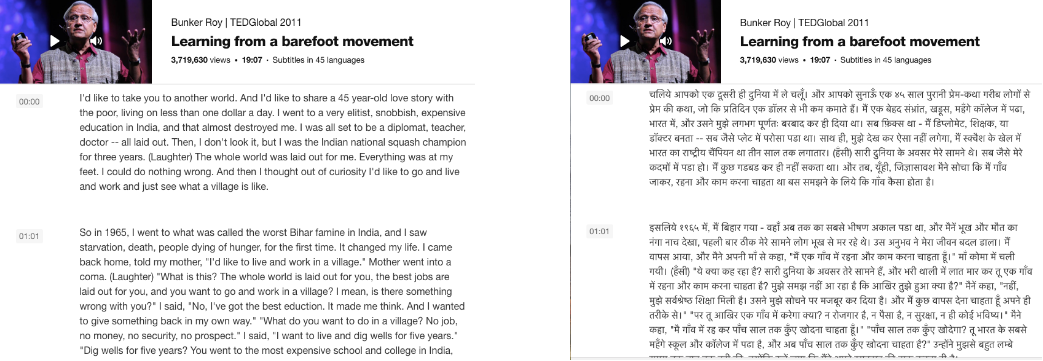
\includegraphics[width=\textwidth]{figures/tedtalks.png}
\caption{A side-by-side figure showing TED Talks\footnotemark  transcripts in English and Hindi} \label{fig1}
\end{figure}
\footnotetext{\url{https://www.ted.com/talks?language=hi},accessed:04.08.2018}
\subsubsection{Beautiful Soup}
Beautiful Soup is one of the most widely used open source Python library designed by Leonard Richardson for quick turnaround projects like website scrapping\citep{bs4}. The decision to use Beautiful Soup for this research was motivated by the fact that It provides simple methods and Pythonic idioms for navigating, searching and modifying a parse tree. It’s a simple toolkit for dissecting the document and extracting the relevant information according to the user’s need. Beautiful Soup makes the handling of encodings much easier, it automatically converts incoming documents to Unicode and outgoing documents to UTF-8. The library sits on top of Popular parsers like lxml and html5lib which allows the user to try different parsing strategies or trade speed for flexibility. 
\subsubsection{Indic NLP Library}
Indic NLP Library\citep{Kunchukuttan2013} is an open source Python based library for common text processing and Natural Language Processing in Indian Languages developed by Anoop Kunchukuttan .  The Indian Languages are originated from Sanskrit and are quite different from the Latin-Based Languages or other Asian Languages, so the other NLP Libraries doesn’t perform well on Indian Languages. Though the Indian languages share a lot of similarity among themselves in terms of script, phonology, language syntax, etc. There are very few researches going in the field of Hindi NLP, and Indic NLP Library is the only existing NLP library for the Hindi language. The library provides several functionalities such as Text Normalization, Tokenization, and Morphological Analysis.
\subsubsection{Moses Tokenizer}
Moses\citep{Koehn:2007:MOS:1557769.1557821} is one of the most successful implementations of the Statistical Machine Translation which was the dominant approach before the onset of Neural Machine Translation. Moses provides several tools for Statistical Machine Translation process, such as for Corpus preparation it provides tokenization, true casing and cleaning tools. As the process of preparation of corpus remains same for Neural Machine Translation Systems, the Moses Tokenizer was chosen here for the tokenization of the English text. The Moses tokenizer was chosen over other tokenizers as the Moses tokenizer is customized for corpus specific tokenization.


\subsubsection{TED Hindi English Corpus}
\begin{figure}
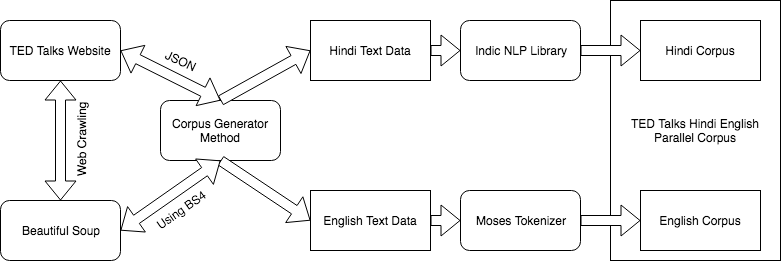
\includegraphics[width=\textwidth]{figures/traindataworkflow.png}
\caption{Workflow of the TED Talks Corpus Generator} \label{fig1}
\end{figure}
TED.com discontinued their Open API project and so there is no direct way to fetch the transcripts of talks. TED.com is a static website, so talks link location is static and can be accessed if prior information of talks details is obtained through Beautiful soup and $urllib$ library in python 

Firstly, the Beautiful Soup library is used to fetch the links of all the 411 TED Talks which are available in the Hindi language from the home page of the TED Official Website. The URL of the web page is passed to the method which implements the Beautiful Soup.  For each and every web page, the $find\_all()$ method finds all the “$a$” tags in the respective pages. Further, $attrs$ method is used to find all the $“href”$ which are having "$/talks$". The URL to the original talks is obtained and stored in a list for further parsing. The method is iterated through the entire list of pages having Hindi TED Talks. 

The transcripts for the talks are fetched from TED’s internal server which is having an open access and URL is appended "$transcript.json?language=en$" . Two different methods for English and Hindi are implemented to obtain the JSON from the respective URLs and load into the data file. 

The JSON is parsed by the respective methods and the transcript text is obtained. The JSON data consisted of time frames, translated text of available language which here Hindi and English respectively. The methods parse the JSON data, fetch the translation and write it in two separate text files “$Hindi.txt$” and “$English.txt$” to create the Hindi-English Parallel Corpus.

The text files generated by the methods were ill-formatted and contained junk texts. So, there was a need for Normalization and Tokenization of the text files. The text written in Hindi displays a lot of quirky behavior on varying input or multiple representations of the same character, so there was a need to canonicalize the representation of the text such that the NLP applications can handle the data inconsistent manner. The canonicalization of the text files handled issues such as,
\begin{itemize}
\item Non-Spacing characters like ZWJ/ZWNL
\item Multiple Representations of Nukta based Characters
\item Multiple Representations of two-part dependent vowel signs
\item Typing inconsistencies such as use of pipe ($|$) for poorna virama 
\end{itemize}

Further the tokenizer in the library was used to tokenize the Hindi text and make it ready for corpora.

The Moses tokenizer comes with two perl scripts  which  is used for normalization and tokenization of the english side of the corpus.

The details of the corpus is showed in Table \ref{corpustable} 

\begin{table}[h!]
\centering
 \begin{tabular}{ |ccc| } 
  \hline Language & Number of Segments & Number of Tokens \\ 
  \hline  Hindi &  84157 & 1412527\\
  English & 84157 & 1407804\\
  \hline
 \end{tabular}
\caption{Details of the TED Talks Hindi-English Corpus}
\label{corpustable}
\end{table}

\subsection{Domain specific Test Data}
\subsubsection{Sumy}
Sumy\citep{belica} is an open source Python library and python command line utility for extracting a summary from HTML pages or plain texts, developed by Miso Belica. The package also contains a simple evaluation framework for text summaries.The decision to use sumy was driven by a number of factors.Sumy is an extractive text summarizer.Extractive text summarization techniques perform summarization by extracting portions of texts and constructing a summary, while the abstractive techniques like Google's TextSum learn the internal language representation to generate more human-like summaries,
and paraphrases the original text. Extractive text summarization makes more sense in the summarization of Blogs as it keeps the original text which highlights the author’s point of view and writing style. Secondly, the abstractive text summarization is technique is highly unfeasible considering the available infrastructure at this stage of research.Further, Sumy provides seven different summarization methods which gives a choice to choose the best summarization algorithm for the blog summarization. 

\subsubsection{Summarizer}

\begin{figure}
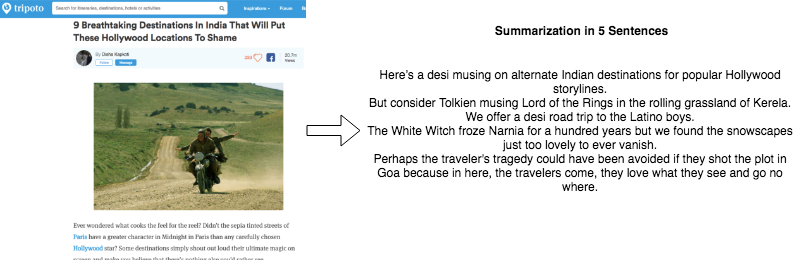
\includegraphics[width=\textwidth]{figures/textsummary.png}
\caption{Figure depicting the summarization of Tripoto Blogs \footnotemark} \label{fig1}
\end{figure}


Tripoto is one of the biggest Travel Blogging Websites in the World. The method implements the Beautiful Soup library and fetches the list of 50 most popular blogs from the URL “$https://www.tripoto.com/trips$ “. The links to the respective blogs is written into a csv (comma separated values) file for the summarization.

The method which implements the sumy library reads the csv file and creates a 5-sentence summary for each and every blog. After experimenting with LexRank, TextRank and Latent Semantic Analysis (LSA), LSA is finally used as the summarizer based on the quality of the summary. The Summary is then saved in a csv file corresponding to their blog links, which is further used by the Visual Interface. The Google Translate API is used to generate the Hindi translation of the summaries which is used as the reference text for evaluation of the translation model. The final domain specific test data consists of 580 pairs of bilingual sentences in Hindi and English.
\footnotetext{\url{https://www.tripoto.com/},accessed:04.08.2018}

\section{Neural Translation Model}
\subsection{PyTorch}
PyTorch is an open source machine learning library for Python developed by \cite{paszke2017automatic}. PyTorch provides high level features like strong GPU acceleration and Dynamic Deep Neural Networks  built on a tape-based autograd system. The decision to use PyTorch was motivated by PyTorch implementation of OpenNMT(\citeauthor{opennmt},\citeyear{opennmt}) which is easily extensible and suitable for research. The decision to use OpenNMT-PyTorch for training the neural model has been discussed in Section \ref{sec:opennmt}.
\subsection{Seq2Seq Model with Attention}
The Seq2Seq model with Attention is well implemented by the OpenNMT Toolkit. The workflow of the English to Hindi Neural Translation Model is showed in Figure \ref{nmtwork}.

\begin{figure}
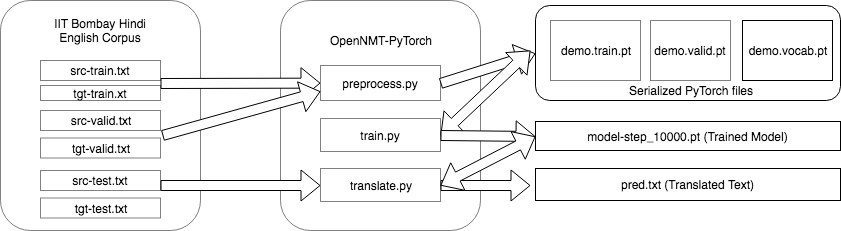
\includegraphics[width=\textwidth]{figures/nmtwork.png}
\caption{Workflow of the Neural Translation Model} 
\label{nmtwork}
\end{figure}

\subsubsection{Pre-Processing} 
Pre-processing is one of the most important component of the Neural Translation Model.The preprocess.py requires the training and validation data from source(english) and target(hindi) language.The validation text files are required by the system to evaluate the converge of training.The preprocess.py is configured according to the design requirements. The size of vocabulary for source and target languages is set to 50K which is well suited for a training data having 1.49 million bilingual sentence pairs.After running the preprocessing.py, the following files are generated by the OpenNMT system:
\begin{itemize}
    \item \textbf{demo.train.pt} A serialized PyTorch file which contains training data.
    \item \textbf{demo.valid.pt} A serialized PyTorch file which contains validation data.
    \item \textbf{demo.vocab.pt} A serialized PyTorch file which contains vocabulary data.
\end{itemize}

These indices are used by the OpenNMT-PyTorch system throughout the process of training and testing. 
\subsubsection{Training}
\label{opennmtmodels}
The Training sub-component consists of train.py which trains the model with the training data from the corpus. The default training configuration consists of 2-layer LSTM with 500 hidden units on both the encoder/decoder. The training component can be configured according to the design requirements. The default word embedding size of 500 for both source and target is maintained throughout the implementation. The training models were implemented using either Bidirectional RNN (\cite{45610}) or LSTMs(\cite{NIPS2014_5346}). \cite{DBLP:journals/corr/VaswaniSPUJGKP17} proposed the Transformer model which is based solely on attention-mechanisms and is different from the tradition Seq2Seq. But the Transformer model was not implemented in this research as the focus was to improve the translations only using LSTM. The following models were implemented using different configurations,
\begin{itemize}
    \item \textbf{OpenNMT-Model-1} Consisted of 4-layer LSTM on the Encoder side, and 4-layer LSTM on the Decoder side, RNN size of 500 units, Attention mechanism as Luong, SGD Optimizer with learning rate of 0.001 and Batch size of 64. 
    \item \textbf{OpenNMT-Model-2} Consisted of 4-layer LSTM on the Encoder side, and 4-layer LSTM on the Decoder side, RNN size of 500 units, Attention mechanism as Luong, Adam Optimizer with learning rate of 0.001 and Batch size of 64. 
    \item \textbf{OpenNMT-Model-3}  Consisted of 2-Layer Bidirectional-RNN on the Encoder side, and 2-layer LSTM on the Decoder side, RNN size of 500 hidden units, Attention mechanism as Luong, SGD Optimizer with learning rate of 0.1 and Batch size of 64. This implementation was motivated by the use of Bi-directional RNN to improve translation quality in Google's NMT (\cite{45610}).
    \item \textbf{OpenNMT-Model-4}  Consisted of 2-Layer Bidirectional-RNN on the Encoder side, and 2-layer LSTM on the Decoder side, RNN size of 500 hidden units, Attention mechanism as Luong, Adam Optimizer with learning rate of 0.001 and Batch size of 64. This implementation was influenced by \cite{DBLP:journals/corr/abs-1712-07628}'s research which concluded that Adam optimizer performs better than SGD in the initial phases of training.
    \item \textbf{OpenNMT-Model-5}  Consisted of 2-Layer Bidirectional-RNN on the Encoder side, and 2-layer LSTM on the Decoder side, RNN size of 1000 units, Attention mechanism as Luong, SGD Optimizer with learning rate of 0.1 and Batch size of 64.\cite{DBLP:journals/corr/BaroneHSHB17} showed that Deep RNNs obtain better translations though they reduce the training speed by significant margin, so the RNN size was increased for this Model.
    \item \textbf{OpenNMT-Model-6} Consisted of 2-layer Bidirectional-RNN on the Encoder side, and 2-layer LSTM on the Decoder side, RNN size of 1000 units, Attention mechanism as Luong, Adam Optimizer with learning rate of 0.001 and Batch size of 64. Its a re-implementation of OpenNMT-Model-5 with Adam optimizer motivated by the performance of Adam optimizer in OpenNMT-Model-4. 
    
\end{itemize}

These models were trained on a Nvidia K80 GPU for 100K steps.The OpenNMT system calculated the training accuracy and perplexity every 50 steps whereas the validation accuracy and perplexity was calculated every 10K steps. The translation models were saved every 5K steps for further re-training. 

\subsubsection{Translating}
The model generated in the previous step is used by translate.py to translate the source text to generate the pred.txt in the target language. The translate.py requires the src-test.txt and the trained model model-step$\_$100000.pt to  translate the source files to the target language. 

\subsection{Back Translation using Monolingual Corpus}
\label{backtrans}
\cite{DBLP:journals/corr/SennrichHB15a} suggested methods for improving the translation quality by making use of monolingual data for low-resource language sources. As discussed before, The IIT-Bombay Hindi Parallel Corpus contains around 1.49 million sentence pairs which is little less for creating optimal neural translation models. This problem can be addressed using the monolingual corpus.\cite{DBLP:journals/corr/SennrichHB15a} suggested two methods to improve the translation quality, first by using dummy source sentences and second, by synthetic source sentences. The results from their experiments showed that the first method is not very efficient and doesn't have much significance on the translation quality. The second method is called back-translation which involves automatic translation of
the monolingual target text into the source language. Then this synthetic source text is paired with the original monolingual target text and added to the human generated parallel training data. The results from their experiments showed that there was substantial improvement on WMT 15 English $\rightarrow$ German translation. 

\begin{itemize}
    \item \textbf{Create back-translations} The main objective in this research is to create English to Hindi translations. For creating backs translations, a new Hindi to English training model is implemented using the same corpus. Then the monolingual sentences are translated using the model. The translations act as synthetic source language data.
    \item \textbf{Re-train using synthetic data} The synthetic data and its equivalent human written monolingual data is integrated for re-training the neural translation model.
\end{itemize}

The IIT Bombay Hindi Monolingual Corpus which is mentioned in \ref{sec:mono} has around 45 million sentences. Creating Back-translations for such a huge monolingual corpus requires huge amount of GPU power which was not feasible for this research work. So, a fraction of the monolingual corpus, 50K sentences were used for creating back translations in English.Then the Hindi monolingual corpus and the English back-translations were integrated with the parallel data for re-training of the model. The detailed workflow of the process is depicted in Figure \ref{backtrans}.

\begin{figure}[h]
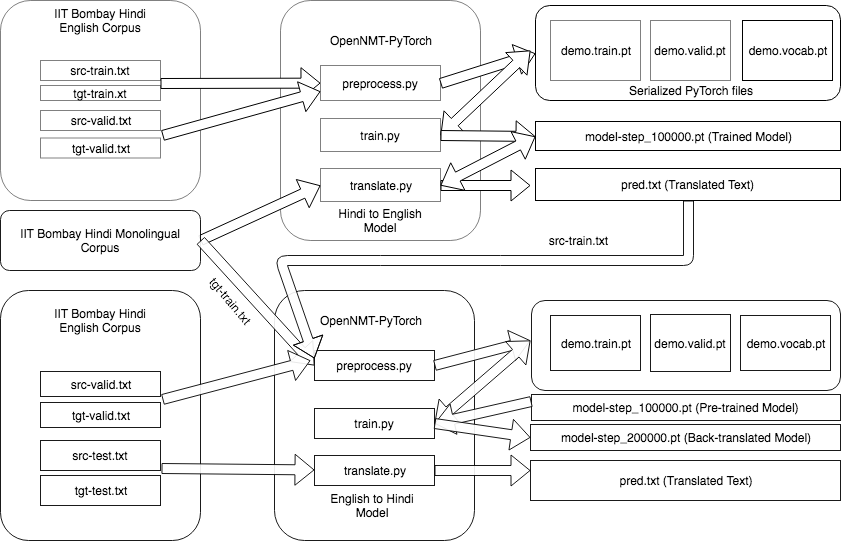
\includegraphics[width=\textwidth]{figures/backtrans.png}
\caption{Workflow of the Back Translation process} 
\label{backtrans}
\end{figure}

\subsection{Fine-Tuning with Cross-Domain Specific Training Data}
The process of fine-tuning involves the re-training of the pre-trained model with cross-domain specific training data. The process is shown in Figure \ref{nmtwork1}. This is a complete re-iteration of the entire training process but with new cross-domain specific data.
\begin{itemize}
    \item \textbf{preprocess.py} The source and target training data from the domain-specific TED Talks Hindi-English Corpus were configured along with validation text from the main IIT-Bombay Hindi-English Corpus.
    \item\textbf{train.py} For the domain specific training with cross-domain specific training data, the configuration of the OpenNMT-Model-6 was implemented.
    \item\textbf{translate.py} The translate.py takes the sentences in the source language and translates them into the target language.
\end{itemize}

\begin{figure}[h]
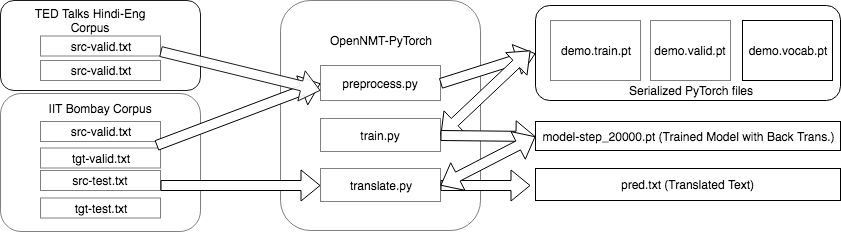
\includegraphics[width=\textwidth]{figures/nmtworkflow1.png}
\caption{Workflow of the fine-tuning process} 
\label{nmtwork1}
\end{figure}

\section{Visual Interface}
The Visual Interface constitutes a simple front end interface component, and is constructed using web application technologies - HTML, CSS, and Javascript to create the static website for visualization.

HTML and CSS are used in combination for mark up and style information. Javascript is used to access the Data Store which contains the translations of the summaries of the blogs.

\subsection{Visual Interface Landing Page}
The landing page, pictured in Figure \ref{display22}, gives brief detail of the motivation of the application, to display the summaries of the blogs in Hindi. The user is presented with a path of action, with clickable selection button.
\begin{figure}[h]
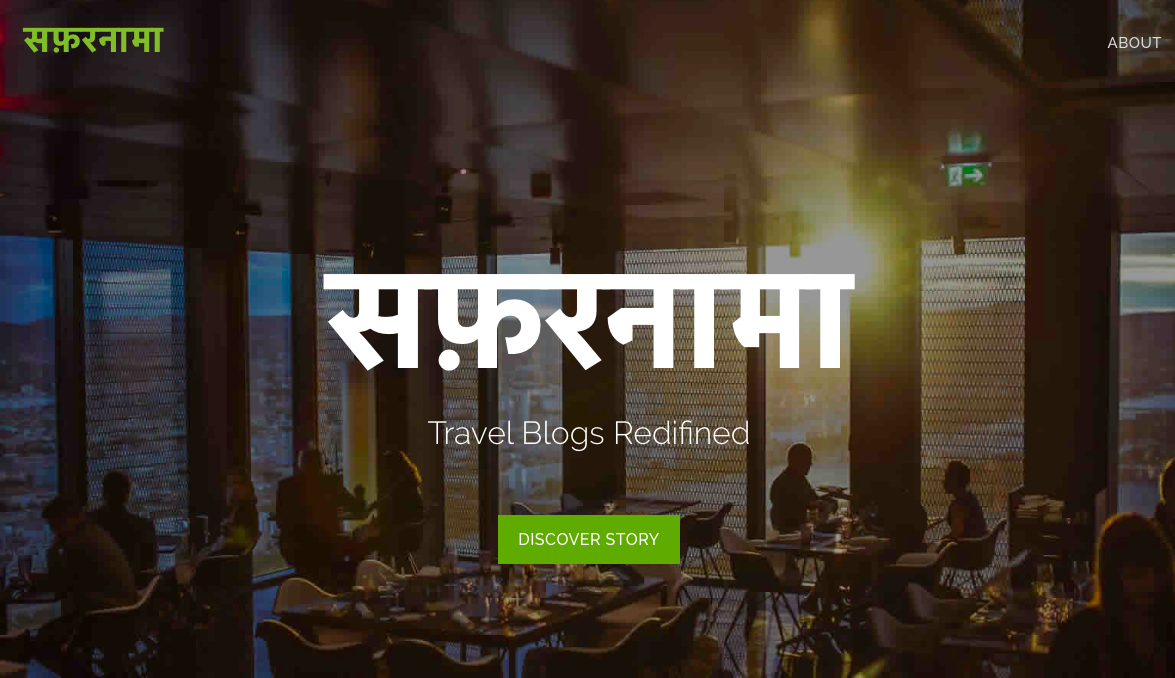
\includegraphics[width=\textwidth]{figures/safarnama1.png}
\caption{Landing page of Visual Interface} 
\label{display22}
\end{figure}

\subsection{Blog Summary Display}

This page, pictured in Figure \ref{display21}, the Blog Summary Display provides options which lets the user to select their interested blogs and the interface pulls the relevant data from the data storage. A five sentence summary of the blog in Hindi and English are displayed on the visual interface. The interface also gives an option to user to further read the blog in the original language English.

\begin{figure}[h]
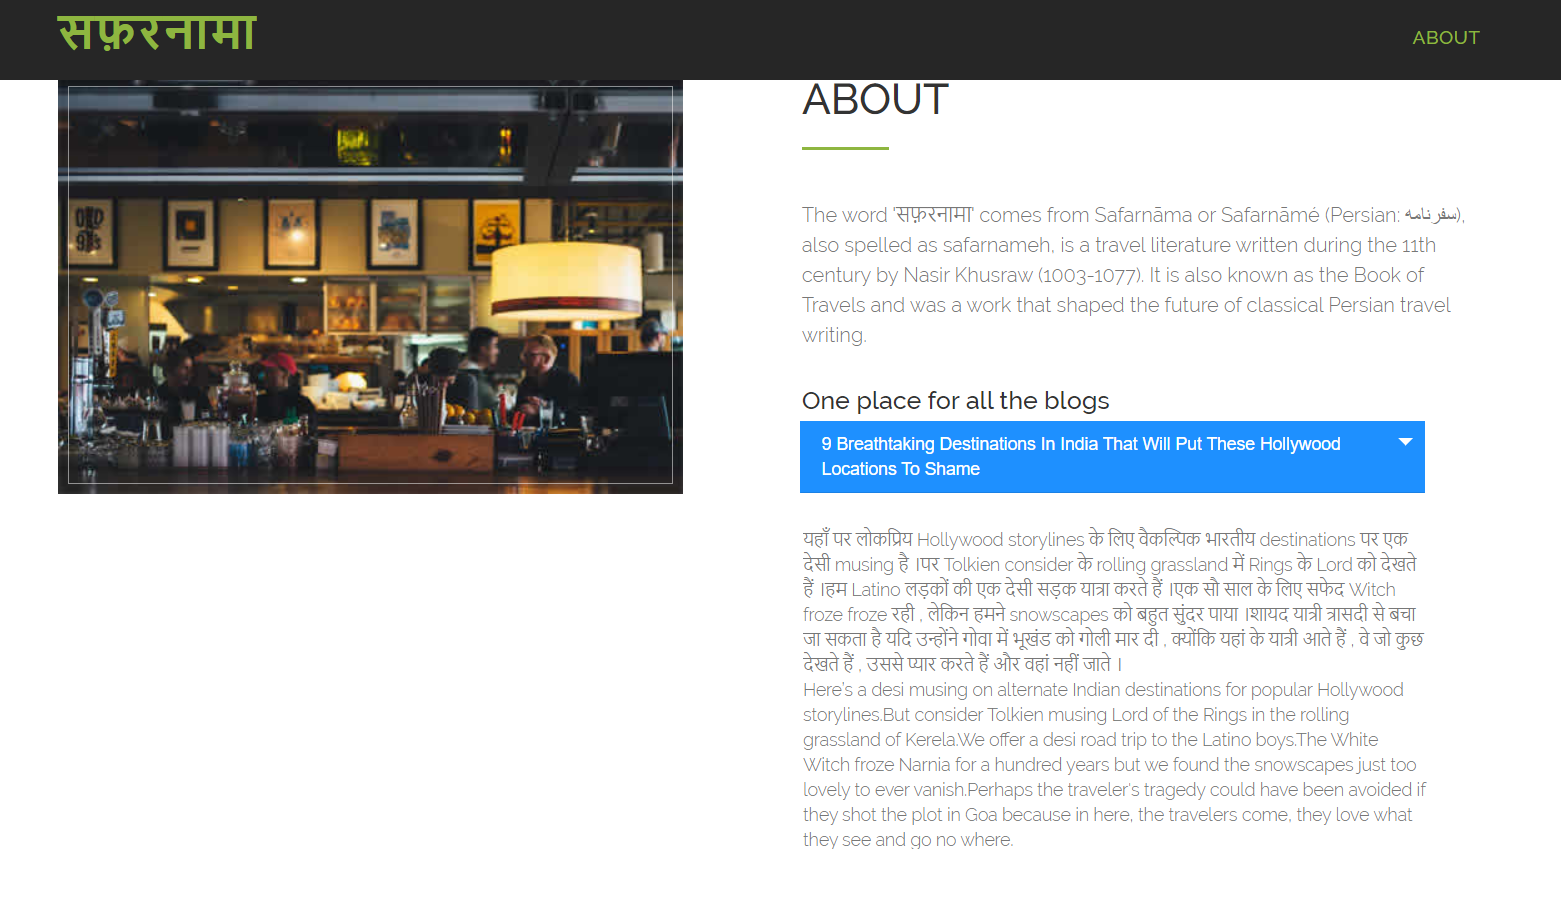
\includegraphics[width=\textwidth]{figures/displaya2.png}
\caption{Blog Summary display} 
\label{display21}
\end{figure}
\section{Summary}
Chapter Four discussed about the various technology decisions made in creating the system. The chapter discussed in details the implementation of domain-specific corpus generation, domain-specific test data generation, neural translation model, and the visualization interface.